\renewcommand{\theequation}{\theenumi}
\begin{enumerate}[label=\thesection.\arabic*.,ref=\thesection.\theenumi]
\numberwithin{equation}{enumi}

\item \solution For $p\brak{x} = x + 5$ 
\begin{flushleft}
The given equation can be represented as follows in the vector form:
\end{flushleft}
\begin{align}
\begin{pmatrix}
5 & -1 
\end{pmatrix}
x + 5 = 0
\end{align}

To find the roots $y=0$:
\begin{align}
x + 5 &= 0 \\
x &= -5
\end{align}
\begin{figure}[!ht]
\centering
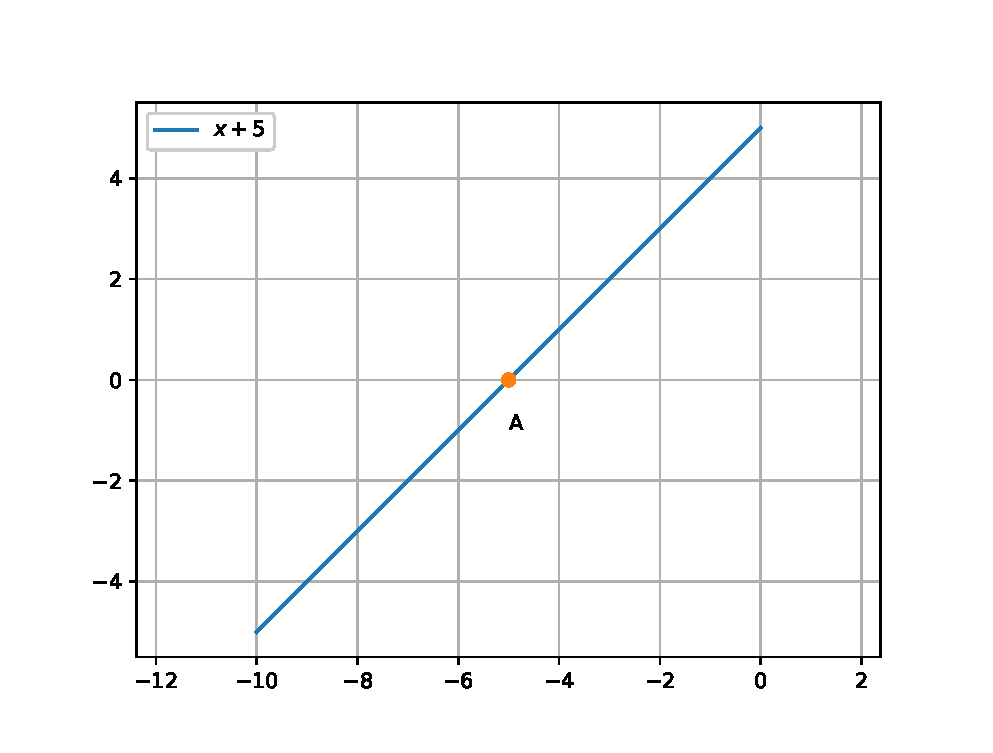
\includegraphics[width=\columnwidth]{./figs/eq1.eps}
\caption{$x + 5$ generated using python}
\label{fig:eq1}
\end{figure} 
%%%%%%%%%%%%%%%%%%%%
\item \solution For $p\brak{x} = x - 5$
\begin{flushleft}
The given equation can be represented as follows in the vector form:
\end{flushleft}
\begin{align}
\begin{pmatrix}
5 & -1 
\end{pmatrix}
x - 5 = 0
\end{align}

To find the roots $y=0$:
\begin{align}
x - 5 &= 0 \\
x &= 5
\end{align}
\begin{figure}[!ht]
\centering
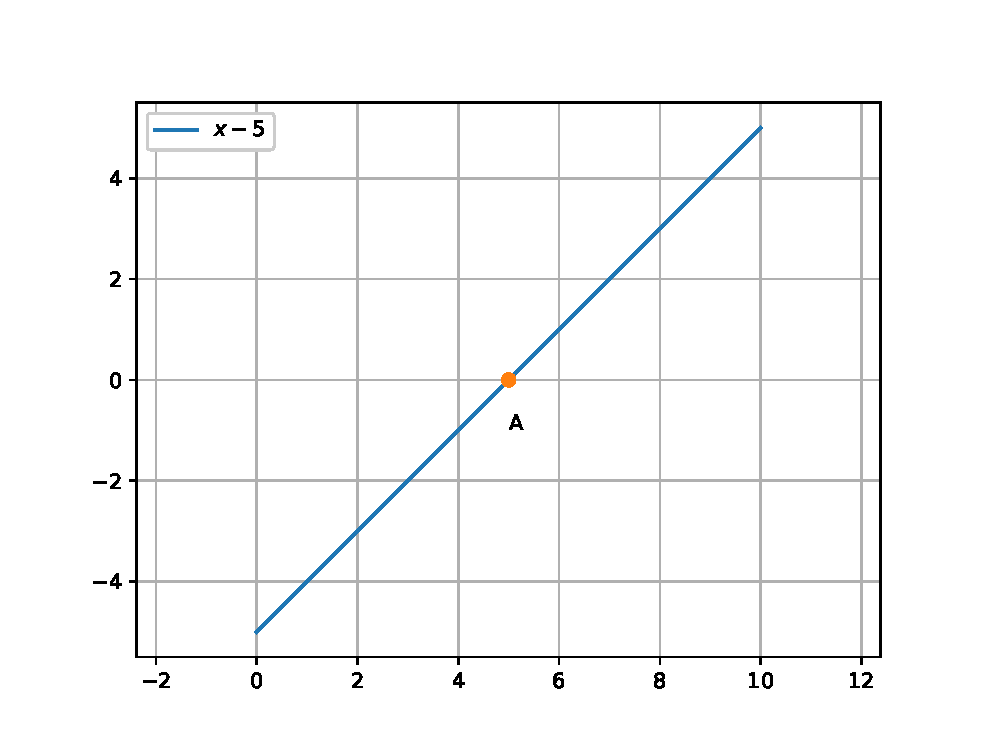
\includegraphics[width=\columnwidth]{./figs/eq2.eps}
\caption{$x - 5$ generated using python}
\label{fig:eq2}
\end{figure}
%%%%%%%%%%%%%%%%%%%%
\pagebreak
\item \solution For $p\brak{x} = 2x + 5$
\begin{flushleft}
The given equation can be represented as follows in the vector form:
\end{flushleft}
\begin{align}
\begin{pmatrix}
2 & -1 
\end{pmatrix}
x + 5 = 0
\end{align}

To find the roots $y=0$:
\begin{align}
2x + 5 &= 0 \\
x &= \frac{-5}{2}
\end{align}
\begin{figure}[!ht]
\centering
\includegraphics[width=\columnwidth]{./figs/eq3.eps}
\caption{$2x + 5$ generated using python}
\label{fig:eq3}
\end{figure} 
%%%%%%%%%%%%%%%%%%%%
\item \solution For $p\brak{x} = 3x - 2$
\begin{flushleft}
The given equation can be represented as follows in the vector form:
\end{flushleft}
\begin{align}
\begin{pmatrix}
3 & -1 
\end{pmatrix}
x - 2 = 0
\end{align}

To find the roots $y=0$:
\begin{align}
3x - 2 &= 0 \\
x &= \frac{2}{3}
\end{align}
\begin{figure}[!ht]
\centering
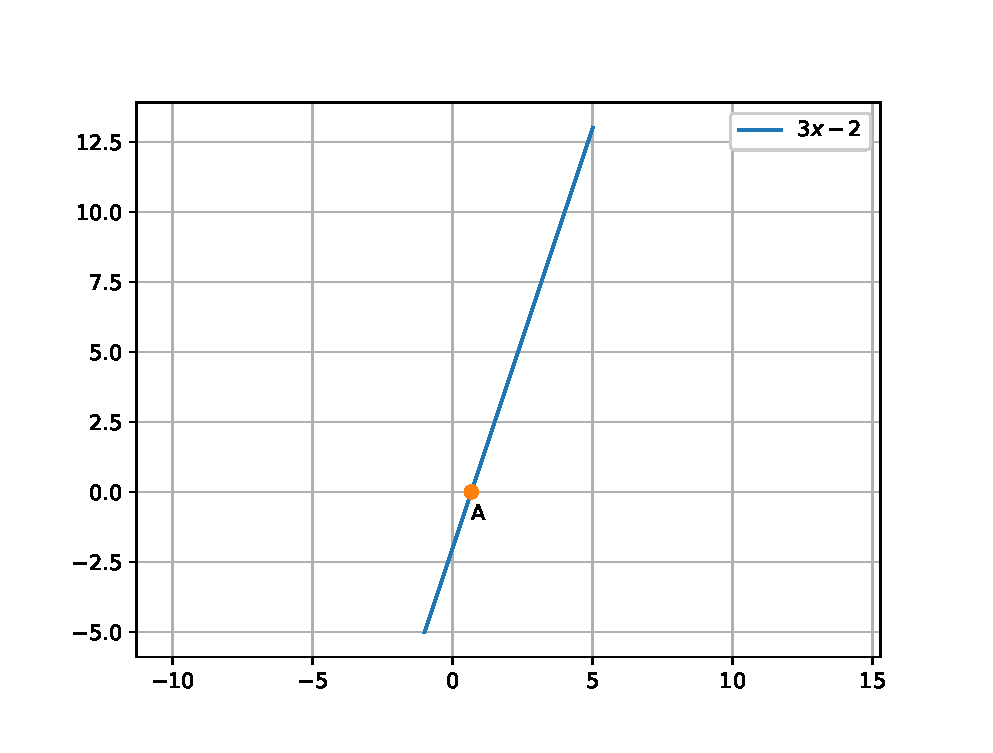
\includegraphics[width=\columnwidth]{./figs/eq4.eps}
\caption{$3x - 2$ generated using python}
\label{fig:eq4}
\end{figure} 
%%%%%%%%%%%%%%%%%%%%
\begin{figure}[!ht] 
\centering
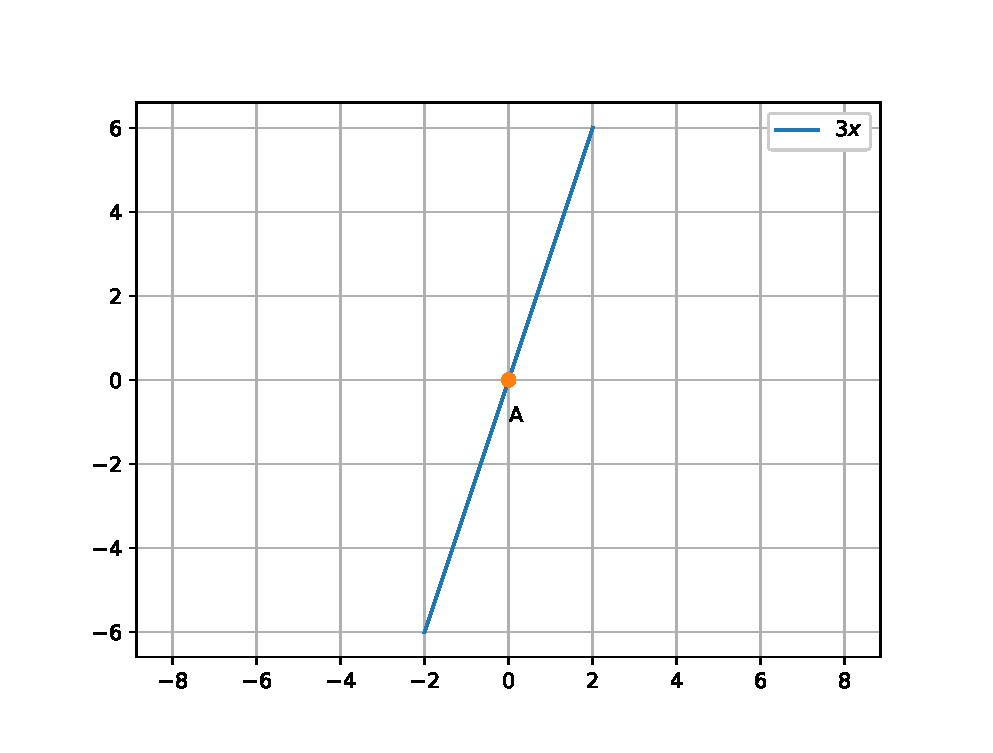
\includegraphics[width=\columnwidth]{./figs/eq5.eps}
\caption{$3x$ generated using python}
\label{fig:eq5}
\end{figure} 
\item \solution For $p\brak{x} = 3x$
\begin{flushleft}
The given equation can be represented as follows in the vector form:
\end{flushleft}
\begin{align}
\begin{pmatrix}
3 & -1 
\end{pmatrix}
x  = 0
\end{align}

To find the roots $y=0$:
\begin{align}
3x  &= 0 \\
x &= 0
\end{align}

\end{enumerate}
